% !TEX root = ../Thesis.tex

\chapter{Introduction}\
\label{ch:introduction}



\section{Motivation and Literature Review}\
\label{ch:motivation}
%(Context and justification, why is this work important?)\\

In December 2015, the COP21 agreement was signed by 195 countries, setting a legally binding goal of reducing greenhouse gasses such as not exceed 1.5\textsuperscript{o}C. The agreement covers accountability, transparency and better reporting of emissions, greater effort towards adaptation and improving the resilience of cities, reducing emissions, and supporting sustainable practices in developing countries. While Europe and other developed countries started introducing building energy requirements since the 1980s, the inclusion of rapidly developing nations with different climates in COP21 creates huge potential for global energy and GHG reductions within the building industry.

\item Improving energy efficiency in buildings does more than just reduce greenhouse gas emissions. It also comes with cost savings and increased earnings for energy exporting countries, improved energy security and higher productivity for businesses\cite{EIA}. In 2014, the global energy efficiency market was worth approximately $USD$90 billion. The projected increase to $USD$125 billion by 2020, which is expected to be driven mainly by energy policy, would still fall short of the $USD$215 billion required to reach just the 2\textsuperscript{o}C target\cite{EIA}. The energy transition in Switzerland, particularly the decision to phase out nuclear energy by 2034, means that maximizing domestic energy efficiency is high on the agenda.

\item Increasing energy efficiency criteria assumes that thermal comfort conditions are met. Efforts toward increasing energy efficiency have led to the re-assessment of comfort theory, from Fanger's PMV model \cite{fanger1970thermal} in the 1970's, typically applied to fully conditioned buildings, to adaptive models now included in ASHRAE standard 55, ISO 7730 and EN15251. These models provide a more realistic representation of comfort in naturally ventilated buildings, in addition to being simpler than the PMV model, since they exploit the linear correlation between comfort temperature and outdoor temperature. 

\item Transposing these models into codes unlocks a great deal of energy saving potential by simply shifting temperature setpoints. However, it is worth bearing in mind when using such ratings that adaptive comfort is also influenced by psychological factors, such as ability to control and adapt to indoor environment, and connection with the outdoors \cite{nicol2002adaptive}. Closed loop building control carries the potential to unlock further system efficiency, and has been the dream , there may be the mistaken temptation to greater automation will have an impact on overall occupant satisfaction and consequently productivity. This notion has implications 

\item Active systems need to be durable

\item 
Energy certification of existing buildings. Performative design of new buildings. Predicting the performance of refurbishments to assess return on investment. Two different types of simulation tools. 
\item
Resistor Capacitor models as used in building physics. Earliest use, subsequent progress. Use in codes
Importance of the stochaistic term \cite{bacher2011identifying}

% \\

%   \begin{figure}[ht] %h can be omitted for better page layout
%     \begin{center}
%       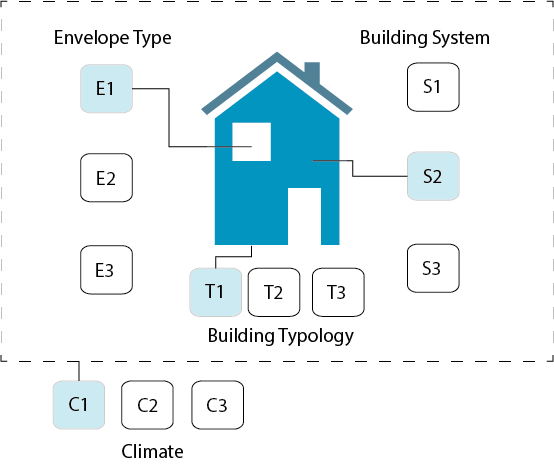
\includegraphics[width=\textwidth, trim= 0cm 0cm 0cm 0cm,clip]{envelope_system_comparison.png}
%       \caption{Figure Example}
%       \label{fig: comparison}
%     \end{center} 
%   \end{figure}

\section{Problem Statement}\
\begin{flushleft}
Because they inherently correct for imperfections and variations in the building fabric, stochaistic models are particularly useful when models need to be fitted to a building whose actual properties are unknown. 

Technologies such as the ASF need robust, accurate models to generate dynamic control inputs in real time.
	\item Simulation of existing buildings for retrofit purposes is time-consuming and not always accurate. An alternative would be a model that uses sensor data to self calibrate
	\item Traditional simulation approach is not good at describing short-time variations, which are important for control applications.
	\item Potential impacts: time savings in design, platform for innovative active integrated systems, more accurate models.
	\item Lack of transparency of source code when wanting to make modifications to test novel building technologies



\section{Objectives of Research}\
%(What do you want to achieve, more in general terms? Bullet point list)\\


	\item  A simple, robust, real-time model is needed to control increasingly complex building-integrated systems.
	\item 
		\item  model predictive control? - would require real-time weather forecasts

	\item  Find the best fitting model to sensor data to avoid running building simulations.

	\item  
		\item  OR: Use sensor data to calibrate adequately accurate model



\begin{itemize}
	\item Review literature and select appropriate models
	\item Set up an 1R-1C thermal model for a single zone as a learning exercise
	\item program 5R-2C thermal models as per ISO codes.
	\item Investigate options for discrete solvers
	
	\item Write good, transferable, open-source code in Python, making the program operable off linux (more reliable)
		\item Manage inputs
		\item output data in a useful and transferable format
	\item Validate the model:
		\item against physical data, possibly ASF and CP, or from existing datasets
		\item Against other models (physics based models) of the same building.
	\item Add complexity:	
		\item Create a graphical interface with a modular R-C model as input
		\item Set up PID controller for actuators (ASF) - requires model for ASF
		\item provide occupancy modelling ... (agent based?)
		\item use computer vision to compute effective window opening factor from photographs of facade and orientation OR just calculate from rhino geometry

\end{itemize}


\section{Thesis Outline}\
%Breakdown of your thesis (Not always necessary)


